\chapter{体积自锁问题}
\section{体积不可压材料}               
考虑一个维度为$n_d$具有边界$\Gamma$的体积不可压材料弹性体$\Omega\in \mathbb R^{n_d}$,其中$\Gamma_t$和$\Gamma_g$分别表示其自然边界和本质边界,
且$\Gamma_t \cup \Gamma_g = \Gamma$, $\Gamma_t \cap \Gamma_g = \varnothing$。该问题相应的强形式为:
\begin{equation}\label{strong_penalty}
    \begin{cases}
        \nabla \cdot \boldsymbol \sigma + \boldsymbol b = \boldsymbol 0 & \mathrm{in} \; \Omega \\
        \boldsymbol \sigma \cdot \boldsymbol n = \boldsymbol t & \mathrm{on} \; \Gamma_t \\
        \boldsymbol u = \boldsymbol g & \mathrm{on} \; \Gamma_g \\
\end{cases}
\end{equation}
其中$\boldsymbol \sigma$为应力张量,对于各向同性线弹性材料,其本构关系表示为:
\begin{equation}\label{stress_penalty}
    \boldsymbol \sigma(\boldsymbol u) = 3\kappa \boldsymbol \varepsilon^v(\boldsymbol u) + 2\mu \boldsymbol \varepsilon^d(\boldsymbol u) 
\end{equation}
式中$\boldsymbol \varepsilon^v$ 和 $\boldsymbol \varepsilon^d$ 为应变张量$\boldsymbol \varepsilon$的体积应变和偏应变部分:
\begin{equation}
    \boldsymbol \varepsilon^v(\boldsymbol u) =\frac{1}{3} \nabla \cdot \boldsymbol u \; \boldsymbol 1, \quad
    \boldsymbol \varepsilon^d(\boldsymbol u) =\frac{1}{2}(\boldsymbol u \nabla + \nabla \boldsymbol u) - \boldsymbol \varepsilon^v, \quad
    \boldsymbol \varepsilon^v : \boldsymbol \varepsilon^d = 0
\end{equation}
其中,$\boldsymbol 1 = \delta_{ij} \boldsymbol e_i \otimes \boldsymbol e_j$是二阶恒等张量。

$\kappa$, $\mu$ 分别为体积模量和剪切模量,它们与杨氏模量$E$和泊松比$\nu$之间存在如下关系式:
\begin{equation}\label{modulus}
    \kappa = \frac{E}{3(1-2\nu)}, \quad \mu = \frac{E}{2(1+\nu)}
\end{equation}
$\boldsymbol b$为$\Omega$中的体力, $\boldsymbol t$, $\boldsymbol g$ 分别为自然边界和本质边界上的牵引力和位移。

对于体积几乎不可压缩材料,它们的泊松比$\nu \rightarrow 0.5$, 相应的体积模量$\kappa \rightarrow \infty$,$\kappa\gg\mu$,使得其体积变化无限小。

采用伽辽金法进行求解时,其相对应的伽辽金弱形式为:
位移$\boldsymbol u \in V$满足
\begin{equation}\label{weak_penalty}
\int_\Omega 2\mu \delta \boldsymbol \varepsilon^d : \boldsymbol \varepsilon^d d\Omega +
\int_\Omega 3\kappa \delta \boldsymbol \varepsilon^v : \boldsymbol \varepsilon^v d\Omega =
\int_{\Gamma_t} \delta \boldsymbol u \cdot \boldsymbol t d\Gamma + \int_\Omega \delta \boldsymbol u \cdot \boldsymbol b d\Omega, \quad
\forall \delta \boldsymbol u \in V
\end{equation}
其中,空间$V=\{\boldsymbol v \in H^1(\Omega)^2\;\vert\;\boldsymbol v = \boldsymbol g, \; \textrm{on} \; \Gamma_g\}$。
$\delta\boldsymbol \varepsilon^v$和$\delta\boldsymbol \varepsilon^d $分别为$\delta \boldsymbol u$表示的体积应变和偏应变的变分。

在传统有限元法中,整个求解域$\Omega$可离散为一组节点$\{\boldsymbol x_I\}_{I=1}^{n_u}$表示\cite{hughes2000},其中$n_u$是位移节点的数量。
位移$\boldsymbol u$及其变分$\delta \boldsymbol u $可通过$\boldsymbol x_I$处的节点系数和形函数进行近似:
\begin{equation}\label{u_h}
    \boldsymbol u_h(\boldsymbol x) = \sum_{I=1}^{n_u} N_I(\boldsymbol x) \boldsymbol u_I, \quad
    \delta \boldsymbol u_h(\boldsymbol x) = \sum_{I=1}^{n_u} N_I(\boldsymbol x) \delta \boldsymbol u_I
\end{equation}
其中$N_I$和$u_I$分别为节点$x_I$处的形函数和节点系数张量。将式\eqref{u_h}代入到弱形式\eqref{weak_penalty}中可得下列的里兹--伽辽金问题:
近似位移 $\boldsymbol u_h \in V_h$满足
\begin{equation}\label{ritz_penalty}
\int_\Omega 2\mu \delta \boldsymbol \varepsilon^d_h : \boldsymbol \varepsilon^d_h d\Omega +
\int_\Omega 3\kappa \delta \boldsymbol \varepsilon^v_h : \boldsymbol \varepsilon^v_h d\Omega =
\int_{\Gamma_t} \delta \boldsymbol u_h \cdot \boldsymbol t d\Gamma + \int_\Omega \delta \boldsymbol u_h \cdot \boldsymbol b d\Omega, \quad
\forall \delta \boldsymbol u_h \in V_h
\end{equation}
其中近似空间$V_h \subseteq V$,$V_h = \{\boldsymbol v_h \in (\mathrm{span}\{N_I\}_{I=1}^{n_u})^{n_d} \vert \boldsymbol v_h = \boldsymbol g,\; \mathrm{on} \; \Gamma_g\}$。
根据$\delta \boldsymbol u_h$的任意性,等式两边同时消除$\delta \boldsymbol u_I$,上述方程可以简化为以下离散控制方程:
\begin{equation}\label{equilibrium_penalty}
    (\boldsymbol K^d +\boldsymbol K^v) \boldsymbol d^u = \boldsymbol f
\end{equation}
式中,体积刚度矩阵$\boldsymbol K^v$ 和偏应力刚度矩阵 $\boldsymbol K^d$的分量分别为:
\begin{equation}\label{stiffness_vol}
    \boldsymbol K^v_{IJ}=  3\kappa\int_{\Omega} \boldsymbol B^{vT}_I \boldsymbol B^v_J d\Omega
\end{equation}
\begin{equation}\label{stiffness_dev}
    \boldsymbol K^d_{IJ}= 2\mu\int_{\Omega} \boldsymbol B^{dT}_I \boldsymbol B^d_J d\Omega
\end{equation}
力向量$\boldsymbol f$的分量为:
\begin{equation}
    \boldsymbol f_I = \int_{\Gamma_t} N_I \boldsymbol t d\Gamma + \int_{\Omega} N_I \boldsymbol b d\Omega
\end{equation}
$\boldsymbol d^u$ 是包含 $\boldsymbol u_I$的系数向量。

对于体积几乎不可压缩的材料,$\kappa \rightarrow \infty$,$\boldsymbol K^v \gg \boldsymbol K^d $。
因此式\eqref{equilibrium_penalty}中的体积刚度矩阵$\boldsymbol K^v$可视作一种强制使用的罚函数法使得体积变形为$0$,即$\nabla \cdot \boldsymbol u = 0$,而体积模量$\kappa$可视作罚因子。
由于这种情况,使用传统有限元法会产生严重的体积锁定,就是所谓的体积自锁现象。

% 1. 约束过多 2. 锁定了K^d的模态,rank(K^d)

\section{调整体积约束}
\subsection{罚函数法}
传统有限元法发生体积自锁的自由度为刚度矩阵的秩$rank(\boldsymbol K)$,通过减少体积刚度矩阵中的积分点数量,可以达到缓解体积自锁的目的。
为了清晰起见,将数值积分代入上述刚度矩阵中:
\begin{equation}
    \boldsymbol K_{IJ} \approx \bar{\boldsymbol K}_{IJ} = \sum_{C=1}^{n_e}\sum_{G=1}^{n_g} \boldsymbol B^{T}_I(\boldsymbol x_G) \boldsymbol B_J(\boldsymbol x_G) w_G
\end{equation}
其中,$\boldsymbol x_G$和$w_G$分别为积分点的位置和权重。$n_e$是单元的数量,$n_g$是每个单元中积分点的数量,因此总的积分点数量为$n_e \times n_g$。

以图\ref{reduced}中二维四边形单元(Quad4)为例,传统二维四边形单元使用$2\times2$高斯积分点作为全积分,对应的体积自锁自由度为:
\begin{equation}
    rank(\boldsymbol K)=min(n_e \times n_g,n_d \times n_u)=min(4n_e,2n_u)
\end{equation}

采用缩减积分单元,积分点的数量从4个减少到1个,此时的体积自由度为:
\begin{equation}
    rank(\boldsymbol K)=min(n_e,2n_u)
\end{equation}
\begin{figure}[H]
    \centering 
    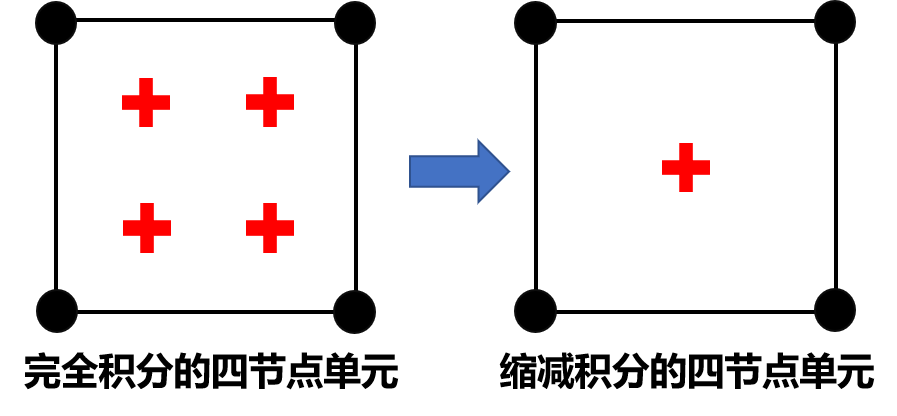
\includegraphics[scale=0.8]{figures/reduced.png}
    \caption{Quad4单元缩减积分}\label{reduced}
\end{figure}
通过减少对体积自由度的约束,缓解体积自锁现象,但是低阶高斯积分将伴随着数值积分精度不足,引起数值计算结果振荡和精度下降。针对低阶高斯积分精度不足的问题,可以使用选择积分法。该方法对于偏应力刚度矩阵使用全积分,
对体积刚度矩阵采用缩减积分进行计算,保持了偏应力刚度矩阵的自由度个数,只减少体积刚度矩阵的自由度个数,从而提高求解精度。

\subsection{拉格朗日乘子法}
施加约束的方式除了传统罚函数法外,还有拉格朗日乘子法。拉格朗日乘子法中将压力$p$作为拉格朗日乘子独立变量,相对应的强形式中增加了压力$p$与位移之间的约束:
\begin{equation}\label{strong_mix}
    \begin{cases}
        \nabla \cdot \boldsymbol \sigma + \boldsymbol b = \boldsymbol 0 & \mathrm{in} \; \Omega \\
        \frac{p}{\kappa} + \nabla \cdot \boldsymbol u = 0 & \mathrm{in} \; \Omega \\
        \boldsymbol \sigma \cdot \boldsymbol n = \boldsymbol t & \mathrm{on} \; \Gamma_t \\
        \boldsymbol u = \boldsymbol g & \mathrm{on} \; \Gamma_g \\
    \end{cases}
\end{equation}
式中应力张量$\boldsymbol \sigma$采用两个变量表示:
\begin{equation}\label{stress_mix}
    \boldsymbol \sigma(\boldsymbol u, p) = p \boldsymbol 1 + 2\mu \boldsymbol \varepsilon^d(\boldsymbol u)
\end{equation}
其中$p\in Q$,$Q = \{q \in L^2(\Omega) \vert \int_{\Omega} q d\Omega = 0\}$。此时,能量泛函具有位移$\boldsymbol u$压力$p$两个变量,分别对两变量进行变分,可得相对应的伽辽金弱形式为:
位移$\boldsymbol u \in V$, 压力$p \in Q$满足
\begin{equation}\label{weak_mix}
    \begin{aligned}
        a(\boldsymbol v, \boldsymbol u) + b(\boldsymbol v, p) &= f(\boldsymbol v) \quad &\forall \boldsymbol v \in V \\
        b(\boldsymbol u, q) &= \boldsymbol 0 \quad &\forall q \in Q
    \end{aligned}
\end{equation}
式中,$a: V\times V\rightarrow \mathbb R$,$b: V\times Q\rightarrow \mathbb R$ 为双线性算子, $f: V \rightarrow \mathbb R$ 为线性算子,它们具有以下形式:
\begin{align}
    a(\boldsymbol v, \boldsymbol u) &= \int_\Omega \nabla^s \boldsymbol v : \nabla^s \boldsymbol u d\Omega \\
    b(\boldsymbol v, p) &= \int_\Omega \nabla \cdot \boldsymbol v p d\Omega \\
    f(\boldsymbol v) &= \int_{\Gamma_t} \boldsymbol v \cdot \boldsymbol t d\Gamma + \int_{\Omega} \boldsymbol v \cdot \boldsymbol b d\Omega
\end{align}

位移$\boldsymbol u$压力$p$双变量可采用不同的离散方式进行近似,形成混合离散框架。
\begin{equation}\label{u_h_mix}
    \boldsymbol u_h(\boldsymbol x) = \sum_{I=1}^{n_u} N_I(\boldsymbol x) \boldsymbol u_I, \quad
    \delta \boldsymbol u_h(\boldsymbol x) = \sum_{I=1}^{n_u} N_I(\boldsymbol x) \delta \boldsymbol u_I
\end{equation}
\begin{equation}\label{p_h_mix}
    p_h(\boldsymbol x) = \sum_{K=1}^{n_p} \Psi_K(\boldsymbol x) p_K, \quad
    \delta p_h(\boldsymbol x) = \sum_{K=1}^{n_p} \Psi_K(\boldsymbol x) \delta p_K
\end{equation}
此时,压力$p$的自由度个数则反应了体积约束个数。式中,$n_p$分别为压力节点的总数,$p_K$为压力节点系数,$\Psi_K$为对应的形函数。

根据$u_h$和$p_h$的任意性,式\eqref{weak_mix}可得到如下离散控制方程:
\begin{equation}\label{equilibrium_mix}
    \begin{bmatrix}
        \boldsymbol K^{uu} & \boldsymbol K^{up} \\ (\boldsymbol K^{up})^T & \boldsymbol K^{pp}
    \end{bmatrix}
    \begin{Bmatrix}
        \boldsymbol d^u \\ \boldsymbol d^p 
    \end{Bmatrix} =
    \begin{Bmatrix}
        \boldsymbol f \\ \boldsymbol 0 
    \end{Bmatrix}
\end{equation}
式中$\boldsymbol K^{uu} = \boldsymbol K^d$. 

由式\eqref{equilibrium_mix}离散控制方程中的第二个等式,系数向量$d^p$可用$d^u$表示:
\begin{equation}
    \boldsymbol d^p = (\boldsymbol K^{pp})^{-1} (\boldsymbol K^{up})^T \boldsymbol d^u
\end{equation}
将上式代入到式\eqref{equilibrium_mix}的第一个等式中可得:
\begin{equation}\label{equilibrium_projection}
    \begin{split}
        &(\underbrace{\boldsymbol K^{uu}}_{\boldsymbol K^d} +  \underbrace{\boldsymbol K^{up}(\boldsymbol K^{pp})^{-1}(\boldsymbol K^{up})^{T}}_{\tilde{\boldsymbol K}^v}) \boldsymbol d^u = \boldsymbol f \\
        \Rightarrow\;& (\boldsymbol K^d + \tilde{\boldsymbol K}^v) = \boldsymbol f
    \end{split}
\end{equation}
此时,位移自由度为$rank(\boldsymbol K^d)$,压力自由度为$rank(\boldsymbol K^v)$。
\begin{equation}
    rank(\boldsymbol K^d)=n_d\times n_u,\quad rank(\boldsymbol K^v)=n_p
\end{equation}

\subsection{罚函数法和拉格朗日乘子法方法的等价性}
从拉格朗日乘子法的离散方程\eqref{equilibrium_projection}中可以看出,压力$p_h$的解是$3\kappa \nabla \cdot \boldsymbol u_h$的一个正交投影。
令$P_h: V_h \rightarrow P_h(V_h)$ 使得 $P_h(V_h) \subseteq Q_h$, 其中 $P_h(V_h) = \textrm{Im}\:P_h$ 是线性算子$P_h$的虚部 \cite{philippeg.2013}. 
在这种情况下, $p_h = P_h (3\kappa \nabla \cdot \boldsymbol u_h) = 3\kappa \tilde \nabla \cdot \boldsymbol u_h$,式\eqref{weak_mix}可以改写为:
\begin{equation}
    \int_\Omega q_h(\nabla \cdot \boldsymbol u_h - \tilde \nabla \cdot \boldsymbol u_h) d\Omega = 0, \quad \forall q_h \in Q_h
\end{equation}
相应的,弱形式体积部分变为:
\begin{equation}\label{projection_mixed}
    \begin{split}
        \int_\Omega \nabla \cdot \delta \boldsymbol u_h p_h d\Omega &= \underbrace{\int_\Omega (\nabla \cdot \boldsymbol u_h - \tilde \nabla \cdot \delta \boldsymbol u_h) p_h d\Omega}_0 + \int_\Omega \tilde \nabla \cdot \delta \boldsymbol u_h \underbrace{p_h}_{\tilde \nabla \cdot \boldsymbol u_h} d\Omega \\
        &= \int_\Omega 3\kappa \tilde \nabla \cdot \delta \boldsymbol u_h \tilde \nabla \cdot \boldsymbol u_h d\Omega \\
    \end{split}
\end{equation}
里兹--伽辽金变分方程变为:
位移$\boldsymbol u_h \in V_h$满足
\begin{equation}
    \int_\Omega 2\mu \delta \boldsymbol \varepsilon^d_h : \boldsymbol \varepsilon^d_h d\Omega +
    \int_\Omega 3\kappa \tilde \nabla \cdot \delta \boldsymbol u_h \tilde \nabla \cdot \boldsymbol u_h d\Omega =
    \int_{\Gamma_t} \delta \boldsymbol u_h \cdot \boldsymbol t d\Gamma + \int_\Omega \delta \boldsymbol u_h \cdot \boldsymbol b d\Omega, \quad \forall \boldsymbol u_h \in V_h
\end{equation}

相比之下,对于罚函数法,缩减积分也可以被视作一种投影。设$\varrho_i$为正交多项式,
\begin{equation}
    \int_{\Omega_C} \varrho_i \varrho_j d\Omega = 
    \begin{cases}
        J_C w_i  & i = j \\
        0 & i \ne j
    \end{cases}
\end{equation}
正交插值 $T^{k}: V \rightarrow W^{k}$,其中 $W^{k}$ 是由$k$个正交多项式构成的插值空间:
\begin{equation}
    W^{k}:= \mathrm{span}\{\varrho_i \}_{i=1}^{k}
\end{equation}
对于传统高斯积分方案,$\varrho_i(\boldsymbol x_j) = \delta_{ij}$, $\boldsymbol x_j$是积分点的位置。体积应变可以通过正交插值法表示为:
\begin{equation}
    \nabla \cdot \boldsymbol u_h(\boldsymbol x) \approx \bar \nabla \cdot \boldsymbol u_h(\boldsymbol x) = \sum_{G=1}^{n_g} \varrho_G(\boldsymbol x) \nabla \cdot \boldsymbol u_h(\boldsymbol x_G), \quad \nabla \cdot \boldsymbol u_h(\boldsymbol x_G) = \bar \nabla \cdot \boldsymbol u_h(\boldsymbol x_G)
\end{equation}
而积分点被视为插值系数。虽然积分点的总数$n_g$低于完全积分,这意味着 $\nabla \cdot \boldsymbol u_h$ 投影到子空间。
\begin{equation}\label{projection_penalty}
    \begin{split}
        \int_\Omega 3\kappa \bar \nabla \cdot \delta \boldsymbol u_h \bar \nabla \cdot \boldsymbol u_h d\Omega
        &= \sum_{C=1}^{n_e} \sum_{G,L=1}^{n_g} 3\kappa \nabla \cdot \delta \boldsymbol u_h(\boldsymbol x_G) \nabla \cdot \boldsymbol u_h(\boldsymbol x_L) \int_\Omega \varrho_G \varrho_L d\Omega  \\
        &= \sum_{C=1}^{n_e} \sum_{G=1}^{n_g} 3\kappa \nabla \cdot \delta \boldsymbol u_h(\boldsymbol x_G) \nabla \cdot \boldsymbol u_h(\boldsymbol x_G) J_C w_G \\
    \end{split}
\end{equation}

通过对比式\eqref{projection_penalty}和式\eqref{projection_mixed},罚函数法实际上与拉格朗日乘子法等价,两种方法都可以用投影的方式来描述。

\section{体积自锁程度判断方法}
\subsection{体积约束比}
约束比是用来衡量变量间的约束程度。对于不可压问题约束比为位移的总自由度比上压力的总自由度。理想情况下,最优约束比应与其偏微分控制方程一致。例如,在二维情况下,不可压问题有两个位移控制方程,一个压力控制方程,所以最优约束比为2.当约束比小于2时会出现体积自锁的倾向。当约束比大于2时会导致压力出现很大的误差。
相关的结论Hughes已经做出了总结\cite{hughes2000}。
\begin{equation}
    r = \frac{n_d\times n_u}{n_p}, \quad 
    \begin{cases}
        r > n_d & \text{过少的约束} \\
        r = n_d & \text{最优} \\
        r < n_d & \text{过多的约束} \\
    \end{cases}
\end{equation}

图\ref{pressure_elements}为四种不同的二维位移压力单元。图(a)为
\begin{figure}[H]
    \centering 
    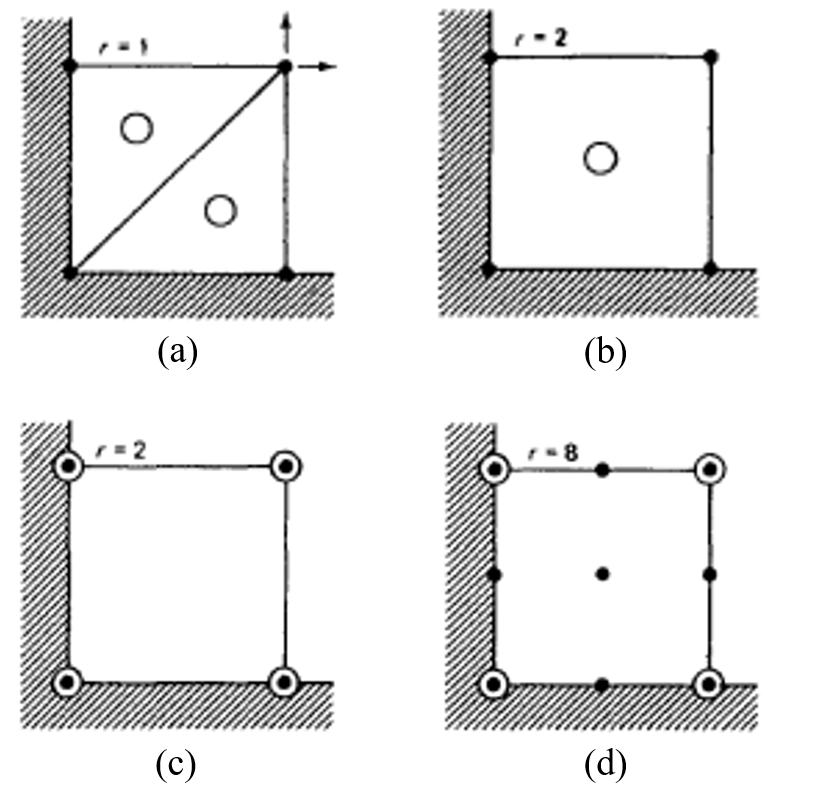
\includegraphics[scale=0.8]{figures/pressure_elements.png}
    \caption{二维位移应力单元示例}\label{pressure_elements}
\end{figure}

从上述结果可以看出,该方法只是一种启发式方法,并不可以精确确定单元组合能否够缓解自锁,只是一种便捷的工具来评估单元是否有缓解自锁的可能,在整体评估单元性能时,还需要考虑其它问题。尽管满足约束比的单元缓解了体积自锁且数值解也比较精确,但它们并非都能满足LBB稳定性条件。
例如Q4P1单元就不满足LBB稳定性条件且压力的解出现了明显的振荡,被称为伪压力模式或应力棋盘模式;
\subsection{LBB稳定性条件}
\begin{equation}\label{infsup}
    \inf_{q_h \in Q_h} \sup_{\boldsymbol v_h \in V_h} \frac{\vert b(q_h,\boldsymbol v_h) \vert}{\Vert q_h \Vert_Q \Vert \boldsymbol v_h \Vert_V} \ge \beta > 0
\end{equation}
